% Use the preamble and structure from guide_tem.tex

\documentclass[a4paper]{article}

% --- Begin guide_tem.tex preamble ---

\usepackage[pages=all, color=black, position={current page.south}, placement=bottom, scale=1, opacity=1, vshift=5mm]{background}
\SetBgContents{
	\tt This work is shared under a \href{https://creativecommons.org/licenses/by-sa/4.0/}{CC BY-SA 4.0 license} unless otherwise noted
}      % copyright

\usepackage[margin=1in]{geometry} % full-width

% AMS Packages
\usepackage{amsmath}
\usepackage{amsthm}
\usepackage{amssymb}

% Unicode
\usepackage[utf8]{inputenc}
\usepackage{hyperref}
\hypersetup{
	unicode,
	pdfauthor={Big Data Research Team},
	pdftitle={Big Data Research System Report},
	pdfsubject={Comprehensive Data Pipeline for COVID-19 Research Analysis},
	pdfkeywords={big data, covid-19, pipeline, analytics, airflow, spark, hadoop, dbt},
	pdfproducer={LaTeX},
	pdfcreator={pdflatex}
}

% Natbib
\usepackage[sort&compress,numbers,square]{natbib}
%\bibliographystyle{mplainnat} % Uncomment if you have references

% Theorem, Lemma, etc
\theoremstyle{plain}
\newtheorem{theorem}{Theorem}
\newtheorem{corollary}[theorem]{Corollary}
\newtheorem{lemma}[theorem]{Lemma}
\newtheorem{claim}{Claim}[theorem]
\newtheorem{axiom}[theorem]{Axiom}
\newtheorem{conjecture}[theorem]{Conjecture}
\newtheorem{fact}[theorem]{Fact}
\newtheorem{hypothesis}[theorem]{Hypothesis}
\newtheorem{assumption}[theorem]{Assumption}
\newtheorem{proposition}[theorem]{Proposition}
\newtheorem{criterion}[theorem]{Criterion}
\theoremstyle{definition}
\newtheorem{definition}[theorem]{Definition}
\newtheorem{example}[theorem]{Example}
\newtheorem{remark}[theorem]{Remark}
\newtheorem{problem}[theorem]{Problem}
\newtheorem{principle}[theorem]{Principle}

\usepackage{graphicx, color}
\graphicspath{{fig/}}

\usepackage{algorithm, algpseudocode}
\usepackage{mathrsfs}
\usepackage{float}
\usepackage{listings}
\usepackage{xcolor}
\usepackage{booktabs}
\usepackage{longtable}
\usepackage{array}
\usepackage{multirow}
\usepackage{wrapfig}
\usepackage{rotating}
\usepackage{caption}
\usepackage{subcaption}
\usepackage{enumitem}
\usepackage{setspace}

% Code listing setup
\lstset{
    basicstyle=\ttfamily\footnotesize,
    breaklines=true,
    frame=single,
    numbers=left,
    numberstyle=\tiny,
    keywordstyle=\color{blue},
    commentstyle=\color{green!60!black},
    stringstyle=\color{red},
    backgroundcolor=\color{gray!10},
    showstringspaces=false
}

% --- End guide_tem.tex preamble ---

% Title and author info
\title{Big Data Research System Report}
\author{Big Data Research Team}
\date{\today}

\begin{document}

\maketitle

\begin{abstract}
This study presents a comprehensive analysis of the Big Data Research System, a sophisticated data pipeline designed for collecting, processing, and analyzing COVID-19 related research data from multiple heterogeneous sources. The system implements a modern big data architecture utilizing cutting-edge technologies including Apache Airflow, Apache Kafka, Apache Spark, Apache Hadoop (HDFS), PostgreSQL, and dbt for data transformation.

The primary objective of this study is to provide real-time insights into COVID-19 related content across news media, social platforms, academic institutions, and video content platforms. The system processes data through a well-defined ETL (Extract, Transform, Load) pipeline, transforming raw data into actionable analytics through a star schema data warehouse design.
\end{abstract}

% --- Begin journal-style factored content ---

\section{Introduction}

The COVID-19 pandemic has generated an unprecedented volume of information across news media, social platforms, academic publications, and video content. Extracting actionable insights from this heterogeneous and dynamic data landscape is a significant challenge for researchers and policymakers. This study addresses this challenge by presenting the Big Data Research System, a comprehensive platform for the real-time collection, processing, and analysis of COVID-19 related data. The main contributions of this study are the design and implementation of a scalable, modular data pipeline that integrates multiple data sources, applies advanced processing and modeling techniques, and delivers interactive analytics through a user-friendly dashboard. The study demonstrates how modern big data technologies can be orchestrated to support timely and reliable research in a rapidly evolving information environment.

\section{Materials and Methods}

The Big Data Research System is architected as a modular pipeline that orchestrates the flow of data from collection to visualization. Data is ingested from a diverse set of sources, including news outlets (Kompas, Detik, NewsAPI, GNews), social media platforms (Reddit, Twitter), YouTube channels (WHO, CDC, academic sources), and academic content from Universitas Gadjah Mada. Python-based scrapers are developed for each source, tailored to the specific structure and requirements of the target platform. These scrapers feed data into an orchestration layer managed by Apache Airflow, which schedules and monitors the execution of the entire pipeline. Real-time data ingestion is facilitated by Apache Kafka, acting as a message broker to decouple data producers from consumers and enable scalable, distributed processing.

Figure~\ref{fig:architecture} shows the high-level architecture of the Big Data Research System. The diagram illustrates the flow of data from various sources through scrapers, orchestration, streaming, processing, storage, transformation, and finally to the dashboard interface. This modular design enables efficient data collection, processing, and visualization in a scalable and maintainable manner.

\begin{figure}[H]
\centering
\resizebox{0.95\textwidth}{!}{%
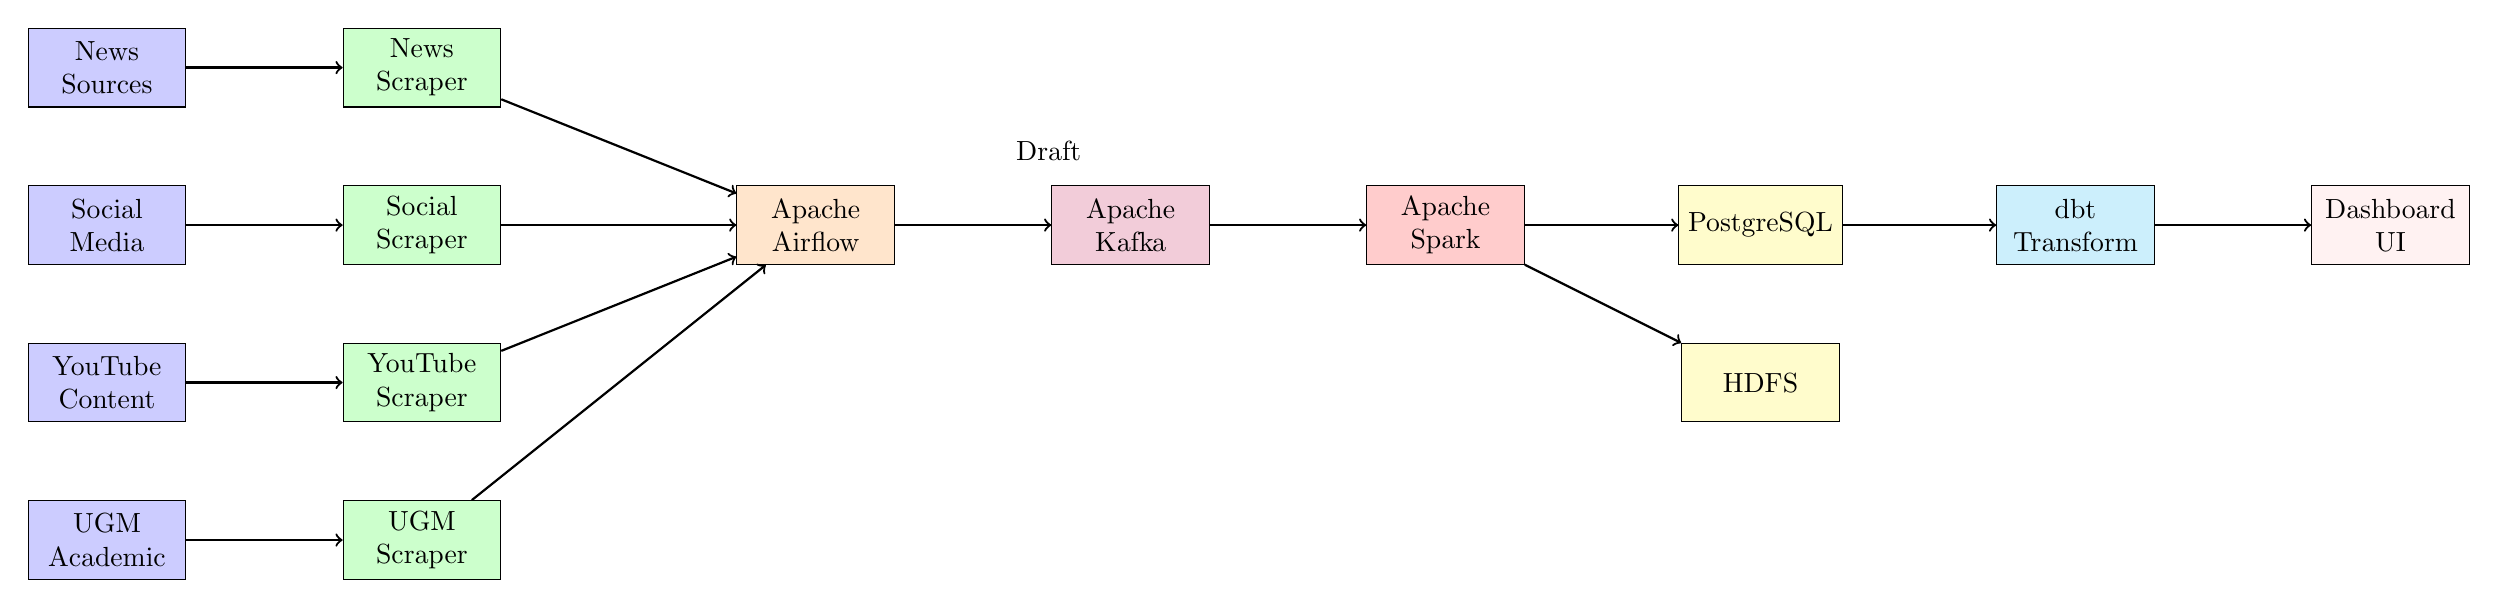
\begin{tikzpicture}[
    node distance=2cm,
    box/.style={rectangle, draw, minimum width=2cm, minimum height=1cm, align=center},
    arrow/.style={->, thick}
]
    % Data Sources
    \node[box, fill=blue!20] (ds1) {News\\Sources};
    \node[box, fill=blue!20, below of=ds1] (ds2) {Social\\Media};
    \node[box, fill=blue!20, below of=ds2] (ds3) {YouTube\\Content};
    \node[box, fill=blue!20, below of=ds3] (ds4) {UGM\\Academic};
    % Scrapers
    \node[box, fill=green!20, right of=ds1, xshift=2cm] (s1) {News\\Scraper};
    \node[box, fill=green!20, right of=ds2, xshift=2cm] (s2) {Social\\Scraper};
    \node[box, fill=green!20, right of=ds3, xshift=2cm] (s3) {YouTube\\Scraper};
    \node[box, fill=green!20, right of=ds4, xshift=2cm] (s4) {UGM\\Scraper};
    % Airflow
    \node[box, fill=orange!20, right of=s2, xshift=3cm] (af) {Apache\\Airflow};
    % Kafka
    \node[box, fill=purple!20, right of=af, xshift=2cm] (k) {Apache\\Kafka};
    % Spark
    \node[box, fill=red!20, right of=k, xshift=2cm] (sp) {Apache\\Spark};
    % Storage
    \node[box, fill=yellow!20, right of=sp, xshift=2cm] (pg) {PostgreSQL};
    \node[box, fill=yellow!20, below of=pg] (hdfs) {HDFS};
    % dbt
    \node[box, fill=cyan!20, right of=pg, xshift=2cm] (dbt) {dbt\\Transform};
    % Dashboard
    \node[box, fill=pink!20, right of=dbt, xshift=2cm] (ui) {Dashboard\\UI};
    % Arrows
    \draw[arrow] (ds1) -- (s1);
    \draw[arrow] (ds2) -- (s2);
    \draw[arrow] (ds3) -- (s3);
    \draw[arrow] (ds4) -- (s4);
    \draw[arrow] (s1) -- (af);
    \draw[arrow] (s2) -- (af);
    \draw[arrow] (s3) -- (af);
    \draw[arrow] (s4) -- (af);
    \draw[arrow] (af) -- (k);
    \draw[arrow] (k) -- (sp);
    \draw[arrow] (sp) -- (pg);
    \draw[arrow] (sp) -- (hdfs);
    \draw[arrow] (pg) -- (dbt);
    \draw[arrow] (dbt) -- (ui);
\end{tikzpicture}%
}
\caption{System Architecture Overview}
\label{fig:architecture}
\end{figure}

The processing layer is powered by Apache Spark, which handles both batch and stream processing tasks. Data is stored in a hybrid storage solution, combining the relational capabilities of PostgreSQL with the distributed storage of HDFS. Data transformation is managed by dbt, which applies SQL-based models to structure the data into a star schema, optimizing it for analytical queries and dashboard consumption. The entire system is containerized using Docker and orchestrated with Docker Compose, ensuring portability and ease of deployment across different environments. Visualization is provided through a Streamlit-based dashboard, offering real-time insights and interactive analytics to end users.

The data pipeline operates on a four-hour schedule, beginning with the parallel execution of all scrapers. Collected data undergoes validation for quality, duplication, completeness, and schema compliance. Validated data is backed up to HDFS and stored in PostgreSQL, with metadata managed for downstream processing. Natural language processing techniques are applied for sentiment analysis, topic classification, keyword extraction, and data aggregation. Spark enables both real-time and batch processing, while dbt structures the transformed data into a star schema and generates analytics tables for dashboard consumption. The pipeline concludes with dashboard refresh and completion notification.

The system employs a star schema data warehouse, with a central fact table capturing COVID-19 mentions and a set of dimension tables providing contextual information about sources, dates, topics, sentiments, and keywords. Figure~\ref{fig:star-schema} shows the star schema data model used in this study. The diagram highlights the relationships between the central fact table and its associated dimension and bridge tables, illustrating how the data is organized to support efficient analytical queries and reporting.

\begin{figure}[H]
\centering
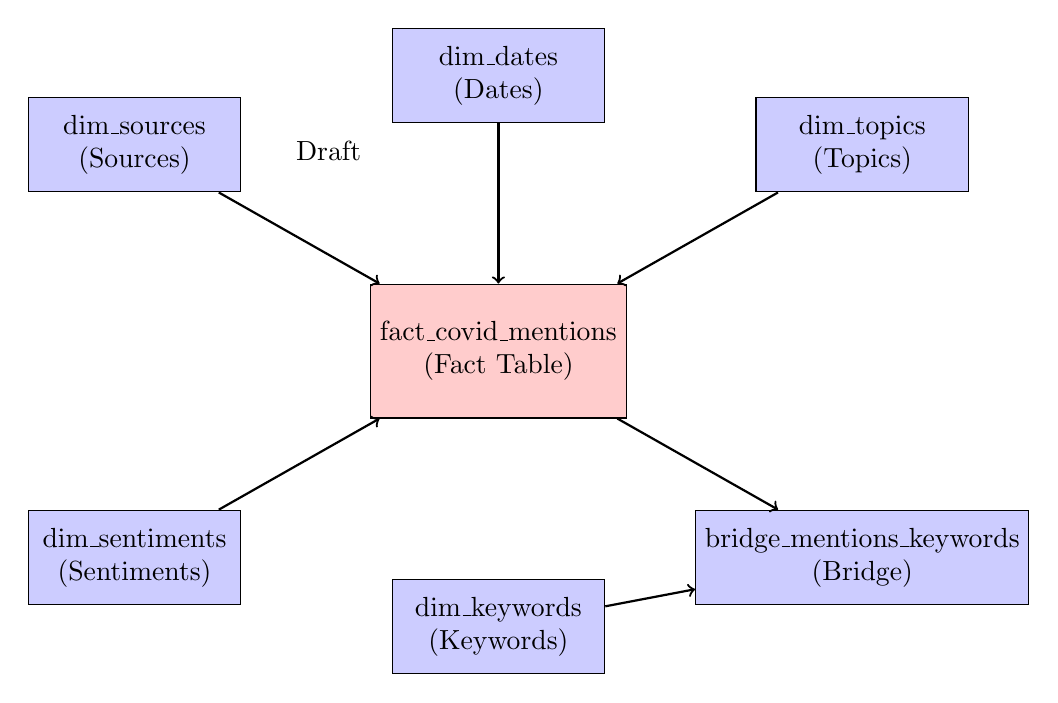
\begin{tikzpicture}[
    node distance=3cm,
    fact/.style={rectangle, draw, fill=red!20, minimum width=3.2cm, minimum height=1.7cm, align=center},
    dim/.style={rectangle, draw, fill=blue!20, minimum width=2.7cm, minimum height=1.2cm, align=center},
    arrow/.style={->, thick}
]
    % Fact Table
    \node[fact] (fact) {fact\_covid\_mentions\\(Fact Table)};
    % Dimension Tables
    \node[dim, above left of=fact, xshift=-2.5cm, yshift=0.5cm] (dim1) {dim\_sources\\(Sources)};
    \node[dim, above of=fact, yshift=0.5cm] (dim2) {dim\_dates\\(Dates)};
    \node[dim, above right of=fact, xshift=2.5cm, yshift=0.5cm] (dim3) {dim\_topics\\(Topics)};
    \node[dim, below left of=fact, xshift=-2.5cm, yshift=-0.5cm] (dim4) {dim\_sentiments\\(Sentiments)};
    \node[dim, below of=fact, yshift=-0.5cm] (dim5) {dim\_keywords\\(Keywords)};
    % Bridge Table
    \node[dim, below right of=fact, xshift=2.5cm, yshift=-0.5cm] (bridge) {bridge\_mentions\_keywords\\(Bridge)};
    % Arrows
    \draw[arrow] (dim1) -- (fact);
    \draw[arrow] (dim2) -- (fact);
    \draw[arrow] (dim3) -- (fact);
    \draw[arrow] (dim4) -- (fact);
    \draw[arrow] (fact) -- (bridge);
    \draw[arrow] (dim5) -- (bridge);
\end{tikzpicture}
\caption{Star Schema Data Model}
\label{fig:star-schema}
\end{figure}

Data processing is orchestrated through a series of Spark jobs, which handle tasks such as batch ETL, data preprocessing, and the application of topic and sentiment analysis models. The system leverages NLP techniques to score sentiment and classify topics, while also extracting keywords and removing duplicate content. Quality scoring is applied to assess the reliability and relevance of each data point. The dbt transformation layer further refines the data, applying a series of SQL models to stage, transform, and aggregate the data for analytical consumption. This layered approach ensures that the data is both accurate and optimized for performance.

\section{Results}

The Big Data Research System delivers a comprehensive dashboard that presents key metrics such as total mentions, daily counts, average sentiment, and the number of active sources. Interactive charts, including line, bar, and pie charts, allow users to explore trends and distributions in the data. A word cloud highlights the most frequently mentioned keywords, while a real-time stream displays the latest data as it arrives. The dashboard is designed to be responsive, ensuring usability across both desktop and mobile devices. The system provides a range of insights, including trend analysis, sentiment analysis, source and keyword analysis, and geographic distribution of content. These outputs support both operational decision-making and strategic research initiatives, enabling users to derive actionable insights from complex and dynamic data sources.

System performance and scalability are achieved through parallel processing, distributed storage, and resource management strategies. Database indexing and caching optimize query performance, while YARN-based resource management ensures efficient allocation of computational resources. The architecture supports horizontal scaling through container-based deployment, with load balancing and fault tolerance mechanisms in place to maintain reliability under varying workloads. Data partitioning strategies further enhance the system's ability to handle large and complex datasets. Data quality is continuously monitored through automated validation checks, with metrics tracked for completeness, accuracy, and consistency. Detailed error logs and performance tracking support ongoing maintenance and optimization efforts.

\section{Discussion}

The results demonstrate that the Big Data Research System is capable of integrating multiple data sources and processing technologies to deliver real-time analytics and high-quality insights. The modular, scalable architecture supports automation, data quality assurance, and user-friendly visualization, making it a valuable tool for researchers and decision-makers. The study highlights the importance of combining modern big data technologies with robust data modeling and processing techniques to address the challenges of heterogeneous and dynamic data environments. Limitations of the current system include the need for ongoing maintenance of scrapers and models as data sources evolve, as well as the potential for further optimization of processing and storage components. Lessons learned from the development and deployment of the system inform recommendations for future enhancements and research directions.

\section{Conclusion and Future Work}

In summary, this study presents a comprehensive solution for the collection, processing, and analysis of COVID-19 data. The Big Data Research System integrates multiple data sources and processing technologies, delivering real-time analytics and high-quality insights through an interactive dashboard. The system's design supports ongoing extension and adaptation, ensuring continued relevance as data sources and analytical needs evolve. Future work will focus on the integration of advanced machine learning models for predictive analytics, the development of real-time alerting systems, the expansion of API capabilities, and the incorporation of deep learning techniques for content analysis. Support for multi-language processing and international content will further broaden the system's applicability, enabling it to address a wider range of research and monitoring challenges in the future.

% Bibliography (uncomment if you have references)
%\bibliography{refs}

\end{document} 